\chapter{Materials and methods}

\section{Initial decisions and simplifications}
From the research that was conducted up to this point, a few key decisions 
could already be made.  

Firstly, as EMG signals seemed to be the most promising for the control of upper 
limb active orthotic devices \cite{dos_santos_signals_2023}, and given the fact 
that a non-invasive system was required, surface EMG (sEMG) sensors were chosen. 
These sensors measure the electrical activity from nerve stimulation at the 
surface of the skin.  

Furthermore, the research revealed that the actuator system best adapted to the 
project requirements would be a system of cables pulled by DC motors. Initially, 
a three-cable system was imagined in order to mimic the three muscles involved 
in elbow flexion: the biceps brachii, the brachioradialis, and the brachialis. 
After consideration of the force produced by each muscle in a single flexion, 
it was concluded that the system can be functional with a single cable. 
Therefore, a single cable-motor system was chosen for simplicity.  

Lastly, 

\section{SysML Models}
\subsection{Context}
\begin{figure}[htbp]
  \centering
  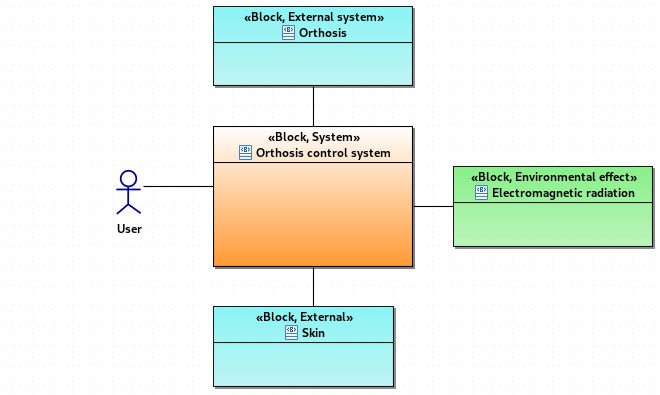
\includegraphics[width=0.8\textwidth]{context.png}
  \caption{Context diagram}
  \label{fig:context_diagram}
\end{figure}
\FloatBarrier
\subsection{Use case}
\begin{figure}[htbp]
  \centering
  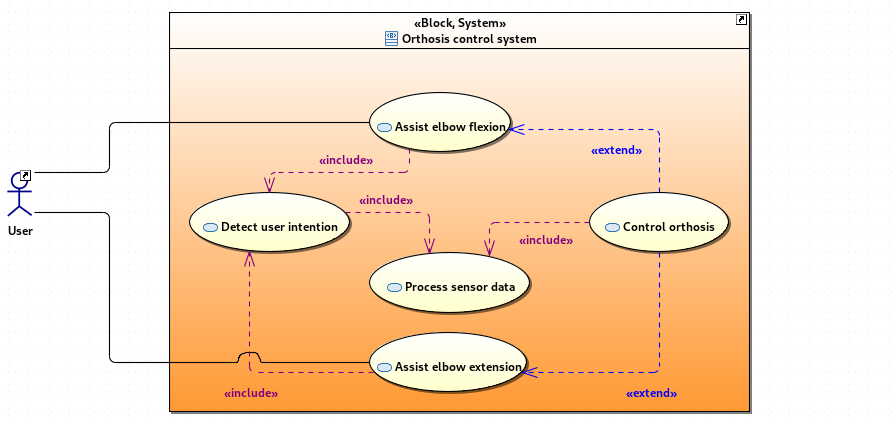
\includegraphics[width=\textwidth]{use_case.png}
  \caption{Use case diagram}
  \label{fig:use_case_diagram}
\end{figure}
\FloatBarrier
\subsection{Requirements}
\begin{figure}[htbp]
  \centering
  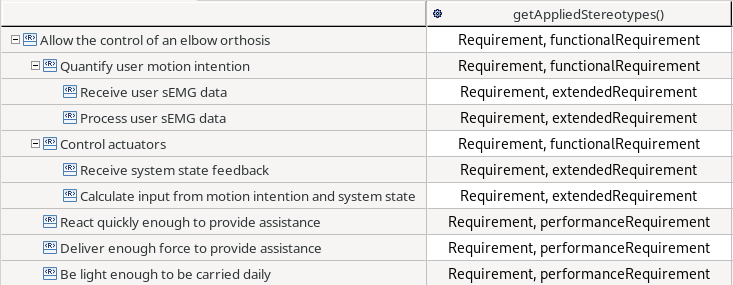
\includegraphics[width=\textwidth]{requirement.png}
  \caption{Requirement table}
  \label{fig:requirements_table}
\end{figure}
\FloatBarrier

\section{Implementation}
A few research papers \cite{lu_development_2019,wu_neural-network-enhanced_2019,wu_adaptive_2023} 
served as guidelines for the project. The goal was to reproduce as much as possible 
from these papers within the project time frame.  

\subsection{Hardware}
The main computer system used to run all programs is a 64bit Linux machine with 
8GB of RAM, a 4-core Intel M-5Y10c @ 2.000GHz and Intel HD Graphics 5300, running 
Fedora 39 (Workstation Edition).  

A FireBeetle 2 ESP32-E was used. Power was supplied by a 3.7V and 400mAh battery 
due to the sensitivity of the analog sEMG sensor.

Two Adafruit BNO055 IMUs were used to measure joint angle, rotation speed 
and acceleration.  

The sEMG sensor initially used was the DataLITE Wireless EMG sensor from Biometrics 
Ltd. However, there was difficulty integrating the sensor with a Linux environment 
as the Biometrics application was only available for Windows machines. Emulation 
through Wine was tested but library dependencies could not be resolved. Therefore, 
another sensor was required. The Myoware Musce Sensor 2 stood out among other options 
as it was used in multiple prior works \cite{lu_development_2019,wu_neural-network-enhanced_2019,
wu_adaptive_2023,russo_algorithm_2018}. As shown in Figure \ref{fig:myoware_processing}, 
this sensor also had the advantage of having built-in signal processing. 

All sensors were connected as shown in Figure \ref{fig:circuit_diagram}. Cables 
were carefully twisted to minimize electromagnetic noise in the sEMG signal.  

The Actuator system was composed of a 150W brushless DC motor from Maxon 
(BLDC-Motor - EC60fl. BL Y 150W 1WE A K) and an EPOS4 Maxon motor driver 
(EPOS4 70/15). Power was supplied by a 3A-30V power supply found at Centrale. 

\begin{figure}[htbp]
  \centering
  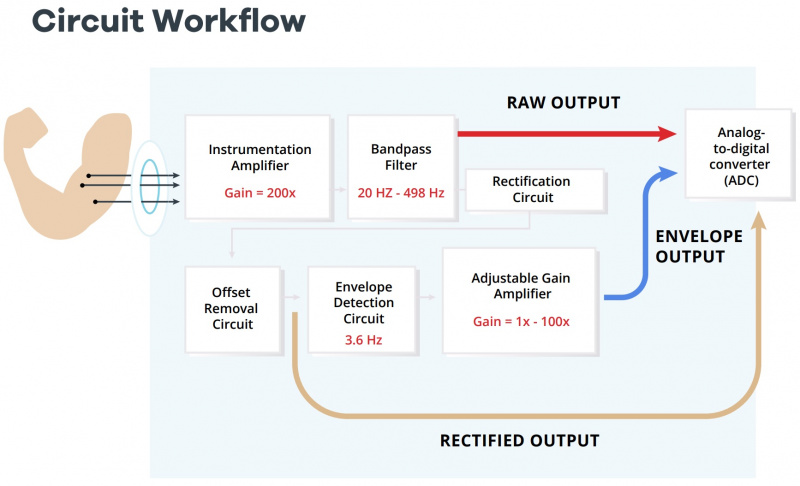
\includegraphics[width=0.8\textwidth]{myoware_processing.jpg}
  \caption{Myoware muscle sensor preprocessing diagram}
  \label{fig:myoware_processing}
\end{figure}
% \begin{figure}
%     \centering
%     \begin{subfigure}{0.3\textwidth}
%         \centering
%         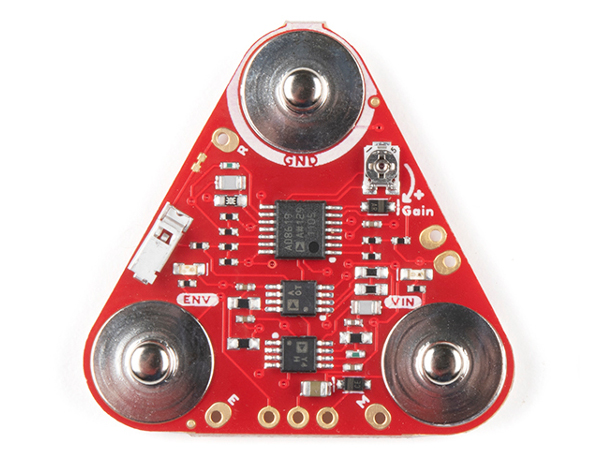
\includegraphics[width=\linewidth]{myoware_sensor.jpg}
%         \caption{Myoware muscle sensor}
%         \label{fig:myoware_sensor}
%     \end{subfigure}
%     \begin{subfigure}{0.2\textwidth}
%         \centering
%         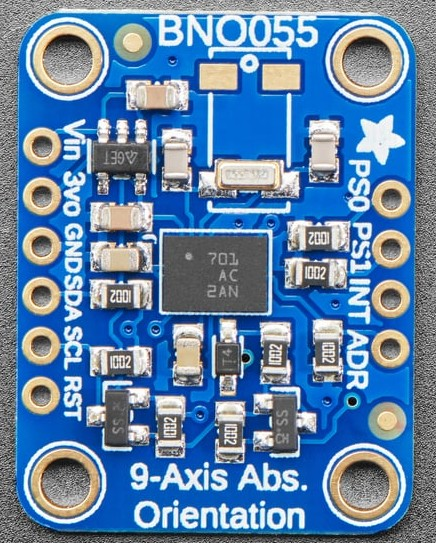
\includegraphics[width=\linewidth]{bno055_sensor.jpg}
%         \caption{BNO055}
%         \label{fig:bno_sensor}
%     \end{subfigure}
%     \begin{subfigure}{0.4\textwidth}
%         \centering
%         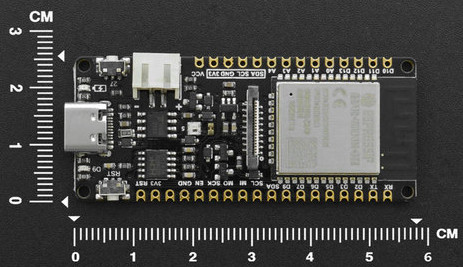
\includegraphics[width=\linewidth]{esp32.jpg}
%         \caption{ESP32}
%         \label{fig:esp32}
%     \end{subfigure}
%     \caption{
%       Sensors and microcontroller
%     }
%     \label{fig:sensor_system}
% \end{figure}
\begin{figure}[htbp]
  \centering
  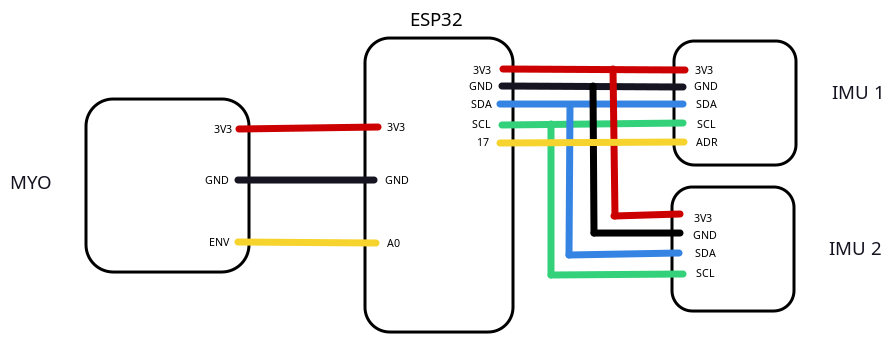
\includegraphics[width=0.8\textwidth]{circuit_diagram.png}
  \caption{Sensor system circuit diagram}
  \label{fig:circuit_diagram}
\end{figure}
\FloatBarrier

\subsection{Control strategy}
A sEMG torque estimation control strategy following the work of Lu et al. 
\cite{lu_development_2019} was put in place. The key difference between the 
control strategy presented in this report and the one presented by Lu et al. 
is that the system output torque is controlled instead of the system angle.  

A version of the control strategy is illustrated in Figure \ref{fig:control_diagram}. 
The sEMG signal gathered from the Myoware muscle sensor (Myo) is fed into a 
torque estimation algorithm that determines user intended torque with a pre-trained 
neural network (NN). Depending on the NN inputs, the control strategy could either be 
open or closed loop.  

In the case of an open loop system, only the user sEMG signal is used to determine 
motion intention and intended torque. That torque is then transformed into required 
motor torque by the orthosis inverse model which is, in turn, transformed into a 
current requirement for motion assistance.  

A closed-loop version could also be considered. In that case, user elbow joint 
angle is also considered in the torque estimation algorithm.  

No force feedback is used because a high degree of accuracy in the assistance 
torque was not considered necessary.  

\begin{figure}[htbp]
    \centering
    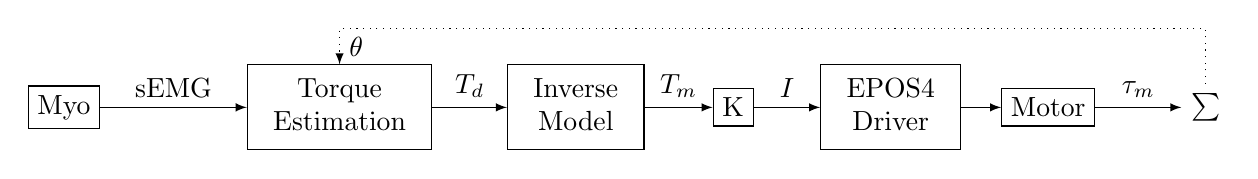
\begin{tikzpicture}[auto, node distance=2cm,>=latex]
        \tikzstyle{block} = [draw, rectangle]
        
        \node [block, draw] (input) at (0,0) {Myo};
        \node [block, draw, right of=input, node distance=3.5cm] (alg) {%
          \begin{tabular}{c}
            Torque\\ 
            Estimation
          \end{tabular}
        };
        \node [block, right of=alg, node distance=3cm] (inv-model) {
          \begin{tabular}{c}
            Inverse\\ 
            Model
          \end{tabular}
        };
        \node [block, right of=inv-model, node distance=2cm] (gain) {K};
        \node [block, right of=gain, node distance=2cm] (driver) {
          \begin{tabular}{c}
            EPOS4\\ 
            Driver
          \end{tabular}
        };
        \node [block, right of=driver, node distance=2cm] (motor) {Motor};
        \node [right of=motor] (sys) {$\sum$};

        \draw [->] (input) -- node[above] {sEMG} (alg);
        \draw [->] (alg) -- node[above] {$T_d$} (inv-model);
        \draw [->] (inv-model) -- node[above] {$T_m$} (gain);
        \draw [->] (gain) -- node[above] {$I$} (driver);
        \draw [->] (driver) -- (motor);
        \draw [->] (motor) -- node[above] {$\tau_m$} (sys);
        \draw [->, dotted] (sys) -- ++(0,1) -| node[near end] {$\theta$} (alg);
        % \draw [->] (sys) -- ++(0,-1) -| node[near end] {$\theta$} (inv-model);
    \end{tikzpicture}
    \caption{
      Control Diagram - $T_d$ designates user desired torque (the torque 
      necessary to perform the movement that the user intends), $T_m$ is the 
      corresponding motor torque required as input to the orthosis system, $\theta$ 
      is the angle of the elbow joint, $K$ is a gain that sets the assistance level 
      of the system and turns $T_m$ into a current requirement $I$
    }
    \label{fig:control_diagram}
\end{figure}

\subsection{Communication strategy}
Establishing a robust communication was essential to ensure reliable data 
transmission between the sensors and processing units. Most of the communication 
was pre-determined by the sensors and equipment. The IMUs communicate via I2C, 
the Myoware sensor outputs an analog value, so is connected to an analog pin 
on the ESP32, and finally the ESP4 driver communicates with the host PC via USB.  

The sensor subsystem, comprised of the two IMUs, the sEMG sensor and the ESP32, 
communicates with the host PC via BLE. This decision was made due to the sensitivity 
of the analog sEMG sensor to outside electromagnetic radiation. Indeed, using 
the sensor while powering the ESP32 by USB produces sub-optimal results. In that 
case, if the PC is charging while using the system, the sensor readings are over 
3600 without any muscle activity. If not charging, the sensor reads correct values 
most of the time but experiences value spikes in the order of 1000, which renders 
the signal unusable. Figure \ref{fig:myo_bug} illustrates this behavior.
It was suspected that imperfections in the PC power supply 
are the cause of these abnormalities, so the choice was made to use a battery. 
BLE was chosen over WiFi or Bluetooth for its advantage on battery life and 
because the data that need to be transferred consist of two numbers every 10-40ms, 
which corresponds to a data rate low enough for BLE. 

\begin{figure}[htbp]
\centering
\begin{circuitikz}[auto,>=latex]
    \node[draw, rectangle] (MC) at (0,0) {ESP32};
    \node[draw, rectangle] (PC) at (3,0) {PC};
    \node[draw, rectangle] (EPOS4) at (7,0) {
          \begin{tabular}{c}
            EPOS4\\ 
            Driver
          \end{tabular}
        };
    \node[draw, rectangle] (Motor) at (10,0) {Motor};
    \node[draw, rectangle] (IMU1) at (0,2) {IMU 1};
    \node[draw, rectangle] (IMU2) at (-3,2) {IMU 2};
    \node[draw, rectangle] (Myo) at (-3,0) {Myo};
    \draw [->] (IMU1) -- (MC) node[midway,right] {I2C};
    \draw (IMU1) -- (IMU2) node[midway,above] {I2C};
    \draw [->] (Myo) -- (MC) node[midway,above] {Analog};
    \draw [->] (MC) -- (PC) node[midway,above] {BLE};
    \draw [<->] (PC) -- (EPOS4) node[midway,above] {Serial};
    \draw (EPOS4) -- (Motor) node[midway,above] {};
\end{circuitikz}
  \caption{System communication diagram}
  \label{fig:communication_diagram}
\end{figure}
\begin{figure}[htbp]
    \centering
    \begin{subfigure}{0.4\textwidth}
        \centering
        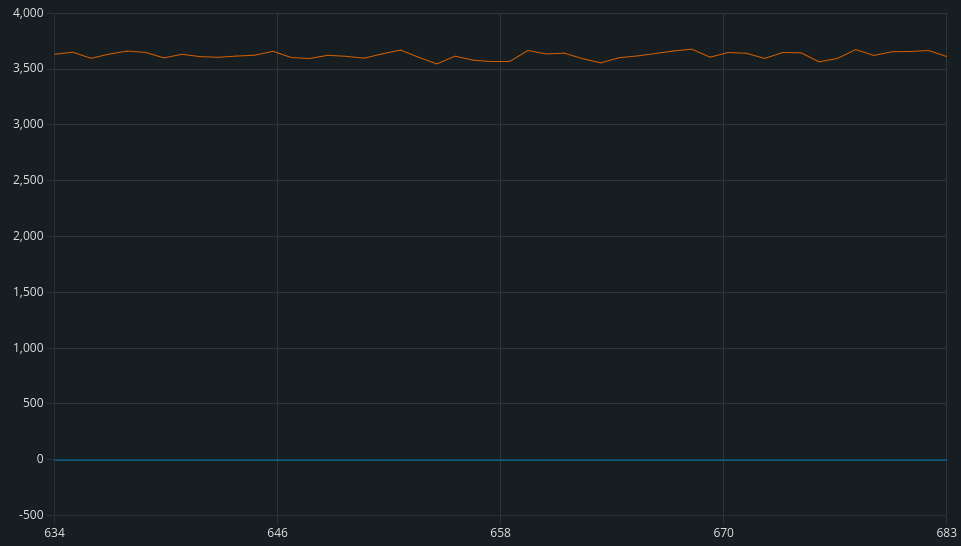
\includegraphics[width=\linewidth]{myo_saturated.png}
        \caption{While PC is charging}
        \label{fig:myo_saturated}
    \end{subfigure}
    \begin{subfigure}{0.4\textwidth}
        \centering
        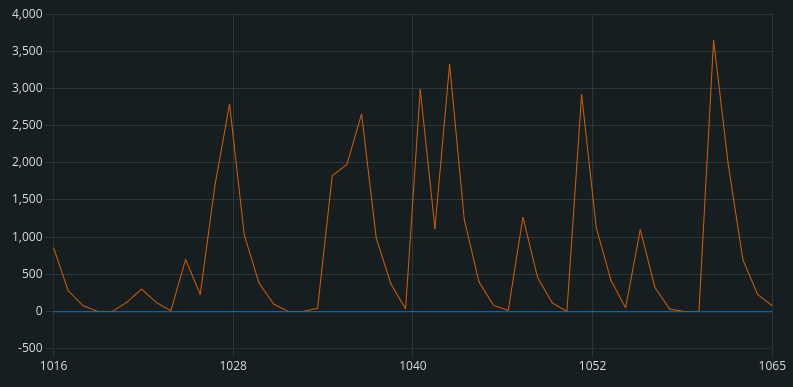
\includegraphics[width=\linewidth]{myo_spikes.png}
        \caption{While PC is not charging}
        \label{fig:myo_spikes}
    \end{subfigure}
    \caption{
      Signal read from the Myoware sensor (orange) while the ESP32 is 
      powered by USB and the biceps muscle is completely relaxed 
    }
    \label{fig:myo_bug}
\end{figure}
\FloatBarrier

\subsection{Software}
Implementing the control strategy required multiple software components to be 
developed. Effort was made to render said software easily comprehensible, 
reusable and upgradeable. A \href{https://github.com/BombVoyage/soft_elbow_orthosis}{Github repository} 
was created to share all code and provide a guide for anyone interested 
in replicating the methods described in this report.  
\subsubsection{Embedded software}
A program that reads sensor data, transforms the IMUs' quaternions 
into a joint angle and sends processed data over BLE was developed for the 
ESP32.  

The $Adafruit\_BNO055$ library was used to acquire data from both IMUs. The ADR 
pin of the first IMU on the I2C bus was set to high to allow for both IMUs to 
be used simultaneously. At each measurement, two quaternions, $q_1$ and $q_2$, 
are obtained. To infer the joint angle, first the relative quaternion $q_r$ 
representing the rotation needed to transform $q_1$ into $q_2$ is calculated, 
then Euler angles $(\psi, \theta, \phi)$ are extracted from $q_r$. The joint 
angle is then identified to one of the obtained Euler angles by experimentation.  

For the sEMG data, the ESP32's A0 pin was simply read.  

Two ways of sending the sensor data were implemented: USB and BLE. The USB 
approach is straightforward but produces undesirable effects on the sEMG sensor 
as discussed in previous sections. The BLE approach involves using the ESP32 
as a BLE server, appropriately named $ESP32\_BLE\_server$, and advertising a 
service with a single characteristic containing both the joint angle and sEMG 
value. 
\FloatBarrier

\subsubsection{Torque estimation}
For torque estimation, a data-driven NN approach was taken.  

Initial data was gathered at INRIA with the help of Yiru Guo and Alyssia Colas. 
Said data consisted of joint angles and sEMG from the biceps brachii muscle. 
Joint angle measurements were made with the Biometrics Ltd. DataLITE goniometer 
and sEMG was measured with the DataLITE sEMG sensor. The data acquisition protocol 
involved performing multiple controlled elbow flexions, covering the entire range 
of motion (ROM) of the joint. Multiple experiments were performed, differing in 
carried load, flexion speed and the presence of pauses in flexion at intermediate 
elbow angles.  

The acquired sEMG data was processed according to the method described by Xu et al. 
\cite{wu_adaptive_2023}: a second order Butterworth filter with a pass-band of 
10-490Hz was used to remove undesirable noise, a 50Hz notch filter was then applied 
to remove power frequency disturbance from nearby equipment and a first order 
Butterworth filter with a high-pass cutoff frequency of 410Hz was applied. Finally, 
the sEMG envelope was obtained with a full-wave rectifier followed by a first order 
Butterworth filter with a low-pass cutoff frequency of 1Hz. The resulting signal 
was then normalized to serve as training data for the NN.  

A sequential NN with a single hidden layer composed of 16 neurons was developed. 
The training and validation data were created from the initial experiments. 
Reference torque was obtained through calculation with the following formula, 
gotten from Lu et al. \cite{lu_development_2019}: 

\begin{align*}
  \tau&=((m+\omega)l_{cm}^2+J)\ddot{\theta}+\beta \dot{\theta}+(ml_{cm}+\omega l)g\sin{\theta}
\end{align*}  

Where $m$ is the mass of the subject forearm and arm, $\omega$ is the mass of 
the carried load, $l$ is the distance from the elbow to the center of the hand,
$l_{cm}$ is the distance from the elbow to the forearm center of mass, $J$ is 
the moment of inertia of the forearm, $g$ is gravitational acceleration and 
$\beta$ is joint friction.  

Four neural network models with identical one hidden layer architecture were trained. 
The initial two models were trained on a singular dataset. One model was trained 
solely on sEMG signals to predict torque, while the other model incorporated angle 
information in addition. These models were labeled as $open\_model$ and $closed\_model$ 
respectively. Subsequently, a second set of models were trained utilizing all 
accessible test data. These models also varied in their inputs akin to the first 
pair. They were denoted as $multi\_open\_model$ and $multi\_closed\_model$ respectively.
\FloatBarrier

\subsubsection{Inverse model}
To calculate the required motor torque $T_m$ from the desired torque $T_d$, 
an inverse model of the orthosis force transmission must be applied. Unfortunately, 
such a model was not available so ideal conditions were considered. The model 
illustrated in Figure \ref{fig:orthosis_model} was used and perfect force 
transmission was hypothesised. The upper arm segment was considered to be along the 
vertical axis for simplicity, i.e. $\psi=0$.  

\begin{figure}[htbp]
    \centering
    \begin{subfigure}{0.2\textwidth}
        \centering
        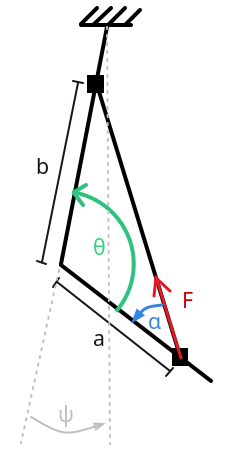
\includegraphics[width=\linewidth]{elbow.png}
        \caption{Elbow model}
        \label{fig:elbow}
    \end{subfigure}
    \begin{subfigure}{0.3\textwidth}
        \centering
        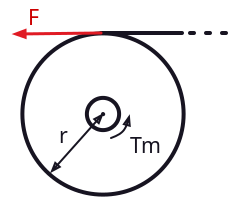
\includegraphics[width=\linewidth]{motor_torque.png}
        \caption{Motor front view}
        \label{fig:motor}
    \end{subfigure}
    \caption{
      Simplified orthosis model
    }
    \label{fig:orthosis_model}
\end{figure}

Let  
\begin{align*}
  R(\theta)=\begin{bmatrix} cos(\theta) & -sin(\theta) \\ sin(\theta) & cos(\theta) \end{bmatrix}
\end{align*}  

Then  
\begin{align*}
  \vec{a}=R(\theta) \cdot \begin{bmatrix} 0 \\ a \end{bmatrix}
\end{align*}  

Therefore  
\begin{align*}
  \vec{T_d} &= \vec{a} \times \vec{F} \\  
  \vec{T_d} &= ||\vec{a}|| \cdot ||\vec{F}|| \cdot \sin(\alpha) \vec{n} \\  
  \vec{T_d} &= ||\vec{a}|| \cdot \left|\left| \frac{\vec{T_m}}{r} \right|\right| \cdot \sin(\alpha) \vec{n} \\  
  ||\vec{T_m}|| &= \frac{r \cdot ||\vec{T_d}||}{||\vec{a}|| \cdot \sin(\alpha)}  
\end{align*}  

Since $\alpha$ is a function of $\theta$, it can be calculated:   

\begin{align*}
  \alpha &= \arcsin(\frac{||\vec{a} \times (\vec{b}-\vec{a})||}{||\vec{a}|| \cdot ||\vec{b}-\vec{a}||}) \\  
\end{align*}  

Finally, we obtain
\begin{align*}
  ||\vec{T_m}|| &= \frac{||\vec{b}-\vec{a}|| \cdot r \cdot ||\vec{T_d}||}{||\vec{a} \times (\vec{b}-\vec{a})||}  
\end{align*}  

Figure \ref{fig:model_1N} illustrates torque predicted by the above model for 
different anchor points of the orthosis cable. 

\begin{figure}[htbp]
  \centering
  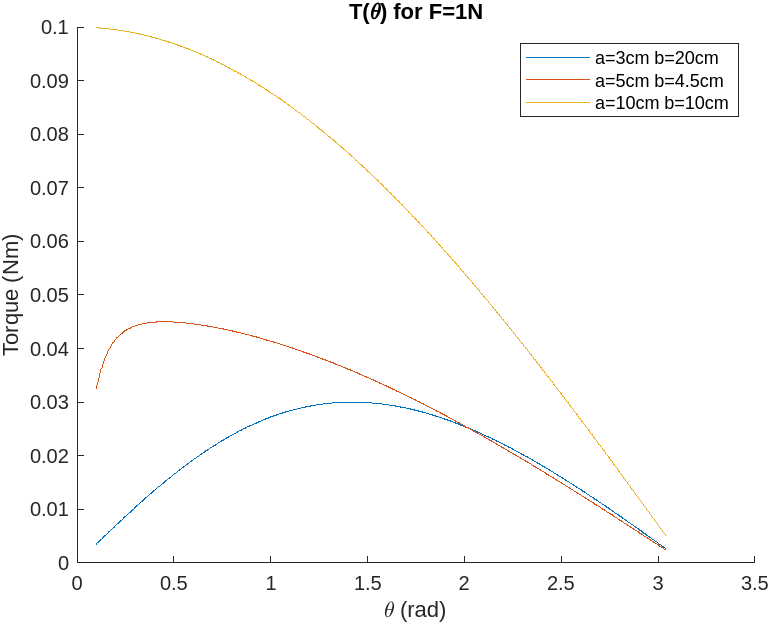
\includegraphics[width=0.8\textwidth]{one_newton_torque.png}
  \caption{Torque generated by 1N of force according to cable anchor points}
  \label{fig:model_1N}
\end{figure}
\FloatBarrier

\subsubsection{Motor driver}
To make use of the EPOS4 70/15 driver, the Linux EPOS Command Library (ECL) was used.  
Three operation modes were developed: current, position and velocity. The position 
and velocity modes serve only for debugging purposes and experimental setup. The driver
is implemented in C, using two threads. A $server$ thread waits for an incoming 
connection and, when established, receives commands for the motor through a socket 
linked to port 8080. Upon reception, a real-time signal containing the command value 
is sent to the $command$ thread. The $command$ thread is responsible for handling 
the real-time signal and using the ECL to control the motor in accordance with the 
chosen mode.  

Originally, the $command$ thread was also responsible for saving data relative to 
the motor's position, velocity and current consumption. However, controlling the 
motor while simultaneously acquiring motor information through the ECL was not 
implemented successfully.  
\FloatBarrier

\subsubsection{Sensor-Motor link}
To link the sensor output to the motor driver, a python program was developed. 
This program first connects to the motor driver's server on port 8080, then 
initiates either a serial or BLE communication with the ESP32, repeatedly reading 
the sensor values. Torque estimation is subsequently performed and by using the 
orthosis inverse model and applying a $K$ gain, the command is finally sent to 
the motor driver.  

Experiment data is saved both as a CSV file and as an image.  
